\chapter{Background}
\label{ch:background}

This chapter provides the background knowledge relevant for the thesis work. It
will present concepts of Computational Complexity
(\autoref{sec:computational_complexity_and_approximability}) and \acrlong{LP}
(\autoref{sec:linear_and_mixed_integer_programming}) as well as graph density problems (\autoref{sec:signed_graphs_and_density}) which are significant in the
following used methodologies.

\section{Computational Complexity and \\Approximability}%
\label{sec:computational_complexity_and_approximability}

Complexity Theory deals with the study of the intrinsic complexity of
computational problems. It also elaborates on the relationships between
the complexity of different problems, for example proving that two problems are
computationally equivalent \cite{9780521884730}, through a notion called
\emph{reduction}.

\subsection{Optimization Problems and $\mathcal{NPO} $}%
\label{sub:optimization_problems}

Optimization problems are defined from a problem instance $x$, a set of
feasible solutions $S$ and a cost function that takes as input the problem
instance $x$ and a feasible solution $s \in S$, denoted as cost$_{O} (x, s) $.
Given a minimization (maximization) problem the optimal solution is defined as
the $s$ minimizing (maximizing) the value of cost$_{O} (x, s)$, and we denote
this value by opt$_{O} (x) $\cite{Trevisan2004}.

\paragraph{$\mathcal{NPO} $}%
\label{par:_npo_}

is then the set of optimization problems with the following properties:
\begin{itemize}
	\item instances $x$ can be recognized in polynomial time;
	\item cost$_{O} (x, s)$ can be computed in polynomial time for $s \in S$;
	\item it takes polynomial time to decide if solution $r$ of the instance
	      $x$ is feasible, i.e.\ whether $r \in S$;
	\item for every instance of the problem $x$
	      and feasible solution for that problem $s \in S$ there is a
	      polynomial $q \; s.t.  \; s \leq q(|x|)$ (i.e. the size of every
	      solution is bounded by a polynomial in $x$).
\end{itemize}

If $\mathcal{P} \neq \mathcal{NP} $ for many optimization problems there is no
algorithm for finding the optimal solution in polynomial time
\cite{Trevisan2004}. This is again a fundamental limitation about what we can
compute which then requires the definition of some alternative approaches, like
\emph{approximation algorithms}
which in polynomial time
compute a solution which lies in a given factor from the optimal
one \cite{Vazirani2002}.

\paragraph{Approximation.}%
\label{par:r_approximations}

$A$ is an r-approximation algorithm for an $\mathcal{NPO} $ minimization
problem $O$ if, for every instance $x$ of $O$ it holds that
\begin{equation*}
	cost_{O} (x, A(x)) \leq r \cdot opt_{O} (x)
\end{equation*}

\noindent
(or, respectively, cost$_{O} (x, A(x))
	\leq 1/r \cdot $opt$_{O} (x) $ for maximization problems), $A(x)$ being the
optimal solution found by the approximation algorithm \cite{Trevisan2004}.

\subsection{Approximation Preserving Reductions}%
\label{sub:approximation_preserving_reductions}

If $\mathcal{N} \neq \mathcal{NP} $ the approximability of problems varies
widely: while for some of them there exist
constant factor approximations, for some others even a remotely approximate
solution cannot be found \cite{Ausiello2005} (some examples are listed in
\autoref{tab:inapproximability-examples}).

\begin{table}
	\centering
	\caption[Examples of inapproximability]{Examples of known inapproximability results, assuming $\mathcal{P}
			\neq \mathcal{NP} $ \cite{10.1007/3-540-63248-4_10} }
	\label{tab:inapproximability-examples}
	\begin{tabular}{c|p{5cm}|c}
		Problem                                                          & Description               & Inapproximability \\
		\hline
		$ \textsc{MaxClique} $                                           & Biggest complete subgraph & $|V|^{1-
		\epsilon}, \epsilon > 0 $                                                                                        \\
		                                                                 &                           &                   \\
		$ \textsc{MaximumIndipendentSet} $                               &
		Biggest set of not connected nodes                               & $|V|^{1-
		\epsilon}, \epsilon > 0 $                                                                                        \\
		                                                                 &                           &                   \\
		$ \textsc{MaxCut} $                                              &
		Partition of nodes in two sets $V_1$ and $V_2$ minimizing the number of edges
		between the 2 sets                                               & 1.0624                                        \\
		                                                                 &                           &                   \\
		$ \textsc{MaximumSetPacking} $                                   & Given a collection of
		finite sets $C$,
		finding the biggest collection $C' \subseteq C$ of disjoint sets & $|C|^{1-
		\epsilon}, \epsilon > 0 $                                                                                        \\
	\end{tabular}
\end{table}

\emph{Approximation preserving reductions} are a fundamental notion for proving
a partial order among optimization problems \cite{Ausiello2005}. Given a
function $f$ mapping instances of $A$ to $B$ and a function $g$ mapping
solutions of $B$ to solutions of $A$, an
approximation preserving reduction must have
the following properties (when reducing from a problem $A$ to a problem $B$)
\cite{DemaineFall2014}:

\begin{itemize}
	\item any instance $x$ of $A$ should be mapped to an instance $x' = f(x)$
	      of $B$ in polynomial time,
	\item any solution $y' \in $ sol$(f(x))$ of $B$ should be associated to a corresponding
	      solution $y = g(x, y') \in $ sol$(x)$ of $A$ in polynomial time.
\end{itemize}

The process is illustrated in \autoref{fig:tex/img/reduction_scheme}.

\begin{figure}
	\centering
	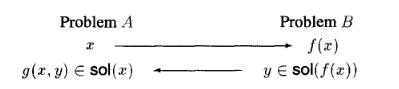
\includegraphics[width=0.6\linewidth]{tex/img/reduction_scheme.png}
	\caption[Reduction process]{The reduction scheme \cite{Crescenzi1997ASG}.}%
	\label{fig:tex/img/reduction_scheme}
\end{figure}

There are at least nine different kinds of approximation preserving reductions
\cite{DemaineFall2014}(\autoref{fig:tex/img/approximation_preserving_reductions}) but we will
focus only on one type.

\begin{figure}[b]
	\centering
	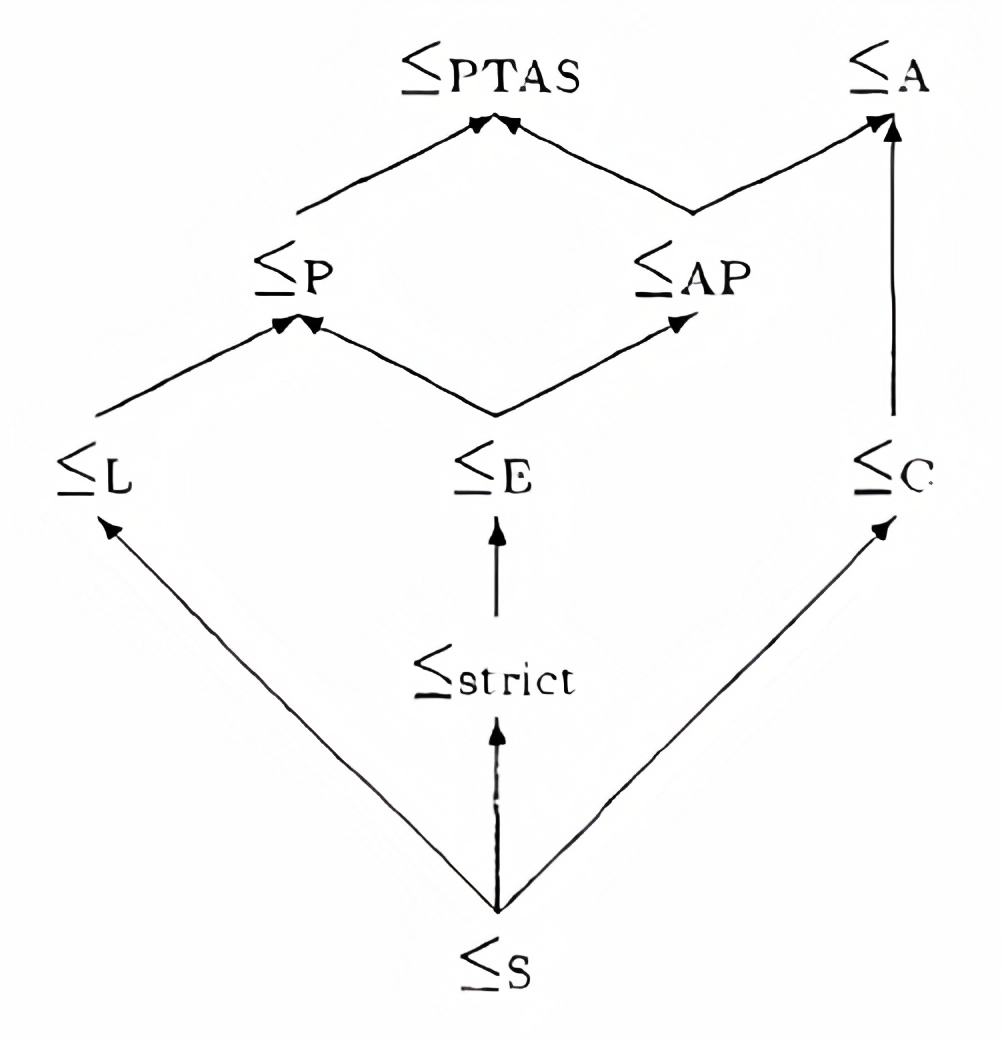
\includegraphics[width=0.4\linewidth]{tex/img/approximation_preserving_reductions.png}
	\caption[Taxonomy of approximation preserving reductions]{Taxonomy of
		approximation preserving reductions \cite{Crescenzi1997ASG}.}%
	\label{fig:tex/img/approximation_preserving_reductions}
\end{figure}

\subsubsection{S Reductions}%
\label{sub:strict_reductions}

An $S$ \emph{reduction} from problem $A$ to problem $B$ has the following properties \cite{Crescenzi1997ASG}:
\begin{itemize}
	\item for any instance $x$ of problem $A$ it holds that opt$_{A} (x) = $
	      opt$_{B} (f(x))$,
	\item for any instance $x$ of $A$ and solution $y'$ of $B$, cost$_{A} (x,
		      g(x, y')) = $ cost$_{B} (f(x), y')$.
\end{itemize}

$S$ reductions are the strongest type of \emph{approximation preserving
	reductions} and imply all the others \cite{Crescenzi1997ASG}.

\section{Linear and Mixed Integer Programming}%
\label{sec:linear_and_mixed_integer_programming}

\acrfull{LP} is a widely used optimization technique and one of the most
effective; the term refers to problems in which both the constraints and \emph{objective
	function} are linear
\cite{Edgar2001,Vanderbei2008,Dantzig1998,Martin1998}. \acrshort{LP}s are solvable in polynomial time \cite{KHACHIYAN198053,Karmarkar1984}.

\subsection{The Structure of \acrshort{LP}s}%
\label{sub:the_structure_of_a_linear_programming_model}

In a \acrshort{LP} problem we are given a vector $ \mathbf{c} = (c_1,
	\dots, c_n) $ and we want to maximize (or minimize) a linear function over
the variables $ \mathbf{x} = (x_1, \dots, x_n) $ with the coefficients of the
vector $ \mathbf{c} $, i.e.
\begin{equation*}
	\mathbf{cx} = \sum^{n}_{i=1} c_i x_i
\end{equation*}
(known as the \emph{objective function}) while satisfying some linear
constraints over the variables \cite{Bertsimas1997,Vanderbei2008}:

\begin{equation*}
	a_1 x_1 + \dots + a_n x_n \begin{Bmatrix} \leq \\ = \\ \geq \end{Bmatrix} b
\end{equation*}

% There is no \emp{a priori} preference regarding how the problem is formulated
% since it is easy to convert an inequality into a equality constraint through
% additional variables ($\omega $ in the example below) called \emph{slack}
% \cite{Vanderbei2008}. For example one in the form
% \begin{equation*}
%     a_1 x_1 + \dots + a_n x_n \leq b
% \end{equation*}
% is equivalent to
% \begin{equation*}
%     a_1 x_1 + \dots + a_n x_n + \omega = b, \quad \omega \geq 0
% \end{equation*}
% and viceversa an equality
% \begin{equation*}
%     a_1 x_1 + \dots + a_n x_n = b
% \end{equation*}
% can be converted into
% \begin{align*}
%     a_1 x_1 + \dots + a_n x_n \leq b \\
%     a_1 x_1 + \dots + a_n x_n \geq b
% \end{align*}
%
In general is possible to formulate any \acrshort{LP} problem as follows (called \emph{standard form}) \cite{Vanderbei2008}

\begin{alignat}{3}
	\label{eq:standard-form}
	\text{maximize}   &       & \sum_{i=1}^{n} c_{i}x_{i}                                          \\
	\text{subject to} & \quad & \sum_{i=1}^{n} a_{1i}  x_{i} & \leq b_{1} &                        \\
	                  &       & \vdots                                                             \\
	                  &       & \sum_{i=1}^{n} a_{mi}  x_{i} & \leq b_{m} &                        \\
	                  &       & x_{i}                        & \geq 0,    & \quad i & =1 ,\dots, n
\end{alignat}


The $x_i$ are known also as \emph{decision variables}; a choice of $ \mathbf{x}
$ is called \emph{solution} and \emph{feasible solution} if it satisfies the
constraints, \emph{optimum} if it \emph{feasible} and maximizes the \emph{objective function}
\cite{Vanderbei2008}.

\subsection{Solving an LP Problem}%
\label{sub:solving_an_lp_problem}

An option for solving an \acrshort{LP} is called the \emph{simplex
	method} which has two different phases.

Starting from the \emph{standard form} \eqref{eq:standard-form}
\emph{slack} variables $x_{n+1}, \dots, $ $x_{n+m} $ are introduced, allowing to express the problem as follows
\cite{Vanderbei2008,Edgar2001}:

\begin{alignat}{3}
	\label{eq:standard-form}
	\text{maximize}   \quad & \sum_{i=1}^{n} c_{i}x_{i}                                                                   \\
	\text{subject to} \quad & x_{n+1}                   = b_{1} - \sum_{i=1}^{n} a_{1i}  x_{i} &                          \\
	                        & \vdots                                                                                      \\
	                        & x_{n+m}                   = b_{m} - \sum_{i=1}^{n} a_{mi}  x_{i} &                          \\
	                        & x_{i}                     \geq 0,                                & \quad i & =1 ,\dots, n+m
\end{alignat}

The first phase involves finding a feasible solution for the problem. More
specifically, we look for $m$ variables, called \emph{basic variables}, whose
value we choose in order to satisfy the $m$ equality constraints (while the
remaining variables, the \emph{nonbasic} ones, are set to 0); if no such
feasible solution exists then the problem is \emph{unfeasible}. Let $\mathcal{B}
$ be the set of \emph{basic variables}, $\mathcal{N} $ the set of
\emph{nonbasic variables} \cite{Vanderbei2008,Bertsimas1997} and
$\bar{\zeta}$ the value of the objective function associated to this feasible
solution. Then the
problem can be reformulated as follows:

\begin{alignat}{3}
	\label{eq:standard-form-simplex-new}
	\text{maximize} \quad     & \bar{\zeta} + \sum_{j \in \mathcal{N} }^{n} c_{j}x_{j}                                           \\
	\text{subject to}   \quad & x_{i} = \bar{b}_{i} - \sum_{j \in \mathcal{N} }^{n} \bar{a}_{ij} x_{j} & \quad i \in \mathcal{B} \\
	                          & x_{i} \geq 0,                                                          & \quad i =1 ,\dots, n+m
\end{alignat}

The second phase of the \emph{simplex method} aims at improving the current
solution: if $c_{j} \geq 0$ for all $j \in \mathcal{N} $, then the value of the
objective function cannot be increased and we found an optimum. If, instead,
there is at least one $c_{j}
	> 0$ then we can increase the value of $\zeta$ by increasing $x_{j} $; now
there are two different cases \cite{Vanderbei2008}:
\begin{itemize}
	\item As $x_{j} $ increases there is at least a variable $\tilde{x}_{j} $
	      whose value needs to decrease to satisfy equality constraints. The first
	      of these variables $\tilde{x}_{j} $ reaching $0$ moves from
	      $\mathcal{B} $ to $\mathcal{N} $, while
	      $x_{j} $ moves from $\mathcal{N} $ to $\mathcal{B} $. The problem is reformulated again as in
	      \eqref{eq:standard-form-simplex-new} and the process is repeated
	      \cite{Vanderbei2008}.
	\item If no such $\tilde{x}_{j} $ variable exists then the value of $x_{j}
	      $ can be increased indefinitely and the problem is said to be
	      \emph{unbounded}, i.e.\ it can achieve any arbitrarily large value.
\end{itemize}

The process is illustrated with an example in \autoref{fig:tex/img/simplex}.

\begin{figure}
	\centering
	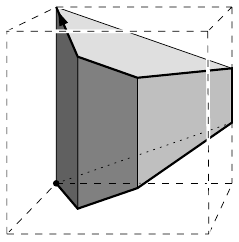
\includegraphics[width=0.4\linewidth]{tex/img/simplex.png}
	\caption[Simplex method progress]{An example of the progress of the \emph{simplex method}: the
		process moves along the vertices of the polygon defined by the
		constraints while improving the value of the solution. Picture taken
		from \cite{BerndGaertner2006}.}%
	\label{fig:tex/img/simplex}
\end{figure}

\subsection{Mixed Integer Programming}%
\label{sub:mixed_integer_programming}

Many problems involve not only continuous variables but also variables that take binary or
integer values: these are known as \acrfull{MIP} problems. Furthermore, some of
these problems are linear in the constraints and in the objective function and are
known as \acrfull{MILP} problems
\cite{Edgar2001,Wolsey1998}.

A generic \acrshort{MILP} can be expressed as follows \cite{Conforti2016}:

\begin{alignat}{3}
	\label{eq:standard-form-milp}
	\begin{aligned}[t]
		\text{maximize}   &                                     & \sum_{i=1}^{n_{1} } c_{i}x_{i} +
		\sum_{i=1}^{n_{2} } h_{i}y_{i}                                                                                                                               \\
		\text{subject to} & \quad                               & \sum_{i=1}^{n_{1} } a_{1i}  x_{i} + \sum_{i=1}^{n_{2} } g_{1i}  y_{i} & \leq b_{1}       &         \\
		                  &                                     & \vdots                                                                                             \\
		                  &                                     & \sum_{i=1}^{n_{1} } a_{mi}  x_{i} + \sum_{i=1}^{n_{2} } g_{1i}  y_{i} & \leq b_{m}       &         \\
		% &       & \sum_{i=1}^{n} a_{mi}  x_{i}                                          & \leq b_{m} &                        \\
		                  &                                     & x_{i}
		                  & \geq 0,                             & \quad i                                                               & =1 ,\dots, n_{1}           \\
		                  &                                     & y_{i}                                                                 & \geq 0,          & \quad i
		                  & =1 ,\dots, n_{2} \; \text{integral}
	\end{aligned}
\end{alignat}

For convenience, we will refer to \acrshort{MILP} problems as \acrshort{MIP} in
the rest of the document.

The \emph{relaxation} of a \acrshort{MIP} problem is defined as the same
problem where the integrality constraints have been removed \cite{Edgar2001}.

Solving a \acrshort{MIP} is a difficult task in general, differently from the
\acrshort{LP} problems. It has been shown also that \acrshort{MIP} is
$\mathcal{NP}$-\textbf{Hard}
\cite{Kannan1978,Liberti2019,Schrijver1998}. This is why the \emph{relaxation} is often considered
for getting an approximation of the exact solution and it can be solved in
polynomial time \cite{Conforti2016}.

\subsection{Solving a MIP}%
\label{sub:solving_a_mip}

One approach that has been proven successful for solving \acrshort{MIP} is the
Branch-and-Bound, which is guaranteed to find an optimal solution
\cite{Conforti2016,Edgar2001}.

Given a problem $P$, the process starts by solving the \emph{relaxation} of $P$
and finding its optimal solution $(\tilde{x}, \tilde{y})$.
Let $S$ and  $\tilde{S}$ be the set of feasible solutions
for the original problem and its relaxation, respectively. By definition,
we have that $S \subseteq \tilde{S} $.
Therefore, \cite{Edgar2001}
\begin{itemize}
	\item If the relaxation problem is not feasible so will be the original
	      problem.
	\item If $\tilde{y}$ has only integer values then we found the optimal
	      solution for the original problem.
	\item If, instead, $\tilde{y}$ contains some fractional values, we start by
	      initializing the value of the best solution so far, $\zeta$, with
	      $-\infty$.  Then we choose one of the fractional variables that are
	      required to be integral in the original problem, say $y_j$ with
	      value $f$, and create two subproblems, respectively adding the
	      constraint $y_{j} \leq \lfloor f \rfloor$ and $y_{j} \geq \lceil f
		      \rceil$. This step is called \emph{branching}. We now consider the
	      solution of each subproblem $(x_j, y_j)$ with value of the objective
	      function $z_{j} $ \cite{Edgar2001,Conforti2016}.

	      \begin{itemize}
		      \item If either of the subproblems is not feasible or its value
		            $z_{j} $ is lower than the best one found so far then it does
		            not need to be considered further. This is called \emph{pruning}.
		      \item If $y_{j} $ are all integer values then $\zeta =
			            z_{j} $.
		      \item Otherwise, we subdivide again in two subproblems as
		            above.
	      \end{itemize}
\end{itemize}


When there are no remaining subproblems to consider then Branch-and-Bound
terminates \cite{Edgar2001}.

\section{Density in Graphs}%
\label{sec:signed_graphs_and_density}

\subsection{The Densest Subgraph Problem}%
\label{sub:densest_subgraphs}

Finding dense subgraphs is a problem which has received a lot of attention and
different definitions of density have been used
\cite{charikar2000greedy,asahiro1995finding,asahiro2000greedily,feige1997densest}.

We will refer to the definition in \cite{charikar2000greedy} and present some
of its results which are used and important for the development of the methods
in the following chapters.

\medskip

Let $G = (V, E)$ be an undirected graph, let $S \subseteq V$ a subset of the
nodes, and let $E(S)$ denote the edges of $G$ induced by $S$, i.e.

\begin{equation*}
	E(S) = \{e_{ij} \in E \; s.t. \; v_i \in S \land \; v_j \in S\}.
\end{equation*}
The \emph{density} $f(S)$ is defined as

\begin{equation}
	f(S) = \frac{|E(S)|}{|S|}.
\end{equation}

According to this definition it is easy to see that $2 \cdot f(S)$ is the
average degree of the subgraph induced by $S$.

The density of the graph $f(G)$ is then defined as

\begin{equation}
	f(G) = \max_{S \subseteq V} {f(S)}.
\end{equation}

The problem of computing $f(G)$ is known as the \emph{Densest Subgraph Problem}
\cite{charikar2000greedy}.

There are different techniques for solving it: a solution based on parametric
maximum flow has been proposed in \cite{Gallo1989}; Charikar in
\cite{charikar2000greedy} proposed an alternative solution based on the
following \acrlong{LP} model (a more in-depth discussion about \acrshort{LP}
can be found in \autoref{sec:linear_and_mixed_integer_programming})

\begin{alignat}{3}
	\label{eq:charikar-model-densest-subgraph}
	\text{maximize}   &       & \sum_{ij \in E} x_{ij}                                          \\
	\text{subject to} & \quad & x_{ij}                  & \leq y_{i} & \quad \forall ij & \in E \\
	                  &       & x_{ij}                  & \leq y_{j} & \quad \forall ij & \in E \\
	\label{eq:charikar-sum}
	                  &       & \sum^{}_{i \in V} y_{i} & \leq 1     &                          \\
	                  &       & y_{i}                   & \geq 0     & \quad \forall i  & \in V \\
	                  &       & x_{ij}                  & \geq 0     & \quad \forall ij & \in E \\
\end{alignat}

Intuitively, the problem associates non-zero $y_i$ to vertices in $S \subseteq V$
and non-zero $x_{ij}$ to edges induced by $S$. The concept of "density" is
introduced by \eqref{eq:charikar-sum}, which distributes a fixed quantity
(one in this case) to the vertices, such that the value $y_i$ of each vertex
generally decreases (and consequently also that of the $x_{ij}$) as the number of non-zero $y_i$ increases.

Let $S(r) \coloneqq \{v_{i} : y_{i} \geq r\} $ and $E(r) \coloneqq \{e_{ij} :
	x_{ij} \geq r\} $. It is easy to see that, given the model as defined
above, $E(r)$ is the set of edges induced by the vertices in $S(r)$.

The set of vertices $S$ maximizing the density $f(S)$ can then be reconstructed
from the results of the \acrshort{LP} by finding the density of $S(r)$
for all choices of $r = y_{i}, \; i \in V $ \cite{charikar2000greedy}.

\paragraph{An approximate algorithm for the Densest Subgraph Problem.}%
\label{par:an_approximate_algorithm_for_the_densest_subgraph_problem}

In \cite{charikar2000greedy}, Charikar also defines a greedy approach for
solving the Densest Subgraph problem which gives a $2$-approximation for
$f(G)$.

The algorithm starts by defining a set of vertices $S$ which is initialized
with $V$ and, through the iterations, it removes from $S$ the vertex $v_i$
which has the lowest degree in the subgraph induced by $S$, until $S$ is empty.
Then it returns the set $S$ which, during the process, was associated with the
highest density $f(S)$.


\subsection{The Densest Common Subgraph Problem}%
\label{sub:the_common_densest_subgraph_problem}

The \acrfull{DCS} Problem was initially introduced by Jethava and Beerenwinke
in \cite{jethava2015finding}
and later studied in \cite{andersson2016finding}, \cite{charikar2018finding}
and \cite{semertzidis2019finding} that also introduced new variants.

\begin{figure}
	\begin{center}
		\begin{subfigure}[b]{0.3\textwidth}
			\centering
			\tikzfig{tex/tikz/graph_history1}
			\caption{$G_1$}
			\label{fig:graph_sequence_example1}
		\end{subfigure}
		\begin{subfigure}[b]{0.3\textwidth}
			\centering
			\tikzfig{tex/tikz/graph_history2}
			\caption{$G_2$}
			\label{fig:graph_sequence_example2}
		\end{subfigure}
		\begin{subfigure}[b]{0.3\textwidth}
			\centering
			\tikzfig{tex/tikz/graph_history3}
			\caption{$G_3$}
			\label{fig:graph_sequence_example3}
		\end{subfigure}
	\end{center}
	\caption[Example sequence graph]{An example of a graph sequence
		$\mathcal{G} = (G_1, G_2, G_3) $ over four vertices.}
	\label{fig:graph_sequence_example}
\end{figure}

Let $\mathcal{G} = (G_1, G_2, \dots, G_T) $ be a sequence of graphs on the same
set of vertices $V$ (an example is shown in
\autoref{fig:graph_sequence_example}), $S \subseteq V$ a
subset of the nodes, $G_i[S]$ the subgraph induced by $S$ in $G_i$,
$\text{deg}_{G_i[S]} (v_{j} )$ the degree of $v_{j} \in S$ in $G_i[S]$ and
$\text{min-deg}(G_i[S])$ the minimum induced degree, i.e.
$\text{min-deg}(G_i[S]) \coloneqq \min _{v_{j}  \in S} \text{deg} _{G_i[S]}
	(v_{j}) $.

Solving the \acrlong{DCS} Problem means finding a subset
of the vertices $S \subseteq V$ that maximizes some aggregate density function
over the graph sequence. More formally, let $g$ be a
function that calculates the density of a set of nodes $S$ in a undirected
graph $G$, i.e.\

\begin{equation*}
	g: S \times G \rightarrow \mathbb{R}.
\end{equation*}

Also, let $h$ be a function aggregating the value of the density of
each snapshot of the graph sequence, i.e.\

\begin{equation*}
	h: g(S, G_1) \times g(S, G_2) \times \dots \times g(S, G_T) \rightarrow
	\mathbb{R}.
\end{equation*}

Then, the \acrshort{DCS} problem consists in finding $S$ maximizing the
following quantity:
\begin{equation*}
	f(S, \mathcal{G} ) = h(\{g(S, G_1 ), \; \dots, \; g(S, G_T) \}).
\end{equation*}

We call $f$ the \emph{density aggregation function}. According to the
definition of $f$ there are different variants
of the problem

\begin{itemize}
	\item \acrshort{DCS}-MM maximizes the Minimum of the Minimum degrees along
	      the graph sequence, i.e.
	      \begin{align}
		      \label{eq:dcs-mm}
		      g & = \text{min-deg} (G_i[S]), & f & = \min_{i \in [T]} \text{min-deg} (G_i[S]).
	      \end{align}
	      A non-trivial solution means finding a set of nodes which are linked
	      in all the graphs $G_i \in \mathcal{G} $.
	      In \cite{semertzidis2019finding} it is shown a simple greedy approach
	      for finding the solution in polynomial time.
	\item \acrshort{DCS}-MA uses the following functions
	      \begin{align}
		      \label{eq:dcs-ma}
		      g        & = \frac{\sum^{}_{v_{j} \in S } \text{deg}_{G_i[S]} (v_{j}
		      )}{|S|}, & f                                                         & = \min_{i \in [T]}
		      \frac{\sum^{}_{v_{j} \in S } \text{deg}_{G_i[S]} (v_{j} )}{|S|}.
	      \end{align}
	      This means finding a set of vertices $S$ which are dense in the sense
	      that they have a non-trivial average degree in all the graphs of the
	      sequence.


	      Charikar, Naamad and Yu in \cite{charikar2018finding} and
	      Semertzidis, Pitoura, Terzi, Tsaparas in
	      \cite{semertzidis2019finding} provide some
	      approximation algorithms with guaranteed bounds;
	      in \cite{charikar2018finding} also they prove its
	      inapproximability to within a $\mathcal{O}(2 ^{\log^{1-\epsilon} n} )
	      $ factor unless $\mathcal{NP} \subseteq \mathbf{DTIME} (n
		      ^{\text{poly}\log n} ) $, $\epsilon > 0$
	      \footnote{They show this results through a reduction from
	      $\textsc{MinRep}$, which has been shown to have the mentioned
	      inapproximability \cite{charikar2018finding,kortsarz2001hardness}.

	      $ \mathbf{DTIME}(f(n)) $ refers to the class of problems that
	      have time complexity $f(n)$ \cite{9780521884730}.
	      }.
	\item \acrshort{DCS}-AM, whose density aggregation function is

	      \begin{equation}
		      \label{eq:dcs-am}
		      f = \sum^{}_{i \in [T]} \text{min-deg} (G_i [S]),
	      \end{equation}
	      while $g$ is the same as in \eqref{eq:dcs-mm}. This choice will push
	      the algorithms to find a set of vertices which have degree greater
	      than $0$ in some of the subgraphs they induce in the graph sequence.

	      Charikar, Naamad and Yu proved in \cite{charikar2018finding}
	      that \acrshort{DCS}-AM is inapproximable within factor $n^{1-\epsilon} $ unless
	      $\mathcal{P} = \mathcal{NP}  $, $\epsilon > 0$
	      \footnote{By reducing from the
		      $\textsc{MaximumIndipendentSet}$ problem.}. For fixed $T$, they also provide a fixed
	      parameter polynomial time algorithm which can be used for solving
	      this problem exactly, as well as a $(1+\epsilon)$-approximation
	      algorithm.
	\item \acrshort{DCS}-AA maximizing

	      \begin{equation}
		      \label{eq:dcs-aa}
		      f = \sum^{}_{i \in [T]} \frac{\sum^{}_{v_{j} \in S} \text{deg}_{G_i[S]}
		      (v_{j} )}{|S|}
	      \end{equation}

	      which puts fewer restrictions than the previous variants on the
	      solutions, requiring only a high average degree on the union of the
	      graphs. Note that $g$ is the same as in \eqref{eq:dcs-ma}.

	      This problem can be solved optimally in polynomial time as it can be
	      reduced to the classical Densest Subgraph problem
	      (\autoref{sub:densest_subgraphs}) \cite{semertzidis2019finding};
	      similarly the approximation algorithm in
	      \autoref{sub:densest_subgraphs}
	      provides a 2-approximation for the optimal solution.

	      More specifically, solving \acrshort{DCS}-AA is the equivalent of solving
	      the \acrfull{DCS} on the average graph $\hat{H}_{\mathcal{G} }  $,
	      which is defined as a weighted graph whose weight of each edge is the
	      fraction of graphs in the sequence $\mathcal{G} $ where the edge is
	      present \cite{semertzidis2019finding}.
\end{itemize}

\subsection{The $\textsc{O}^{2} \textsc{Bff}$ Problem}%
\label{sub:the_o_2_bff_problem}

The \acrshort{DCS} is also known as the \acrfull{BFF} Problem as defined by Semertzidis, Pitoura, Terzi, Tsaparas
\cite{semertzidis2019finding}; in the same paper also another class of similar
problem is defined, the \acrlong{O2BFF} Problem.

Let $\mathcal{G} = (G_1, G_2, \dots, G_T) $ be a sequence of graphs on the same
vertex set $V$. The \acrfull{O2BFF} is defined as the set of
vertices $S \subseteq V$ and the set of $k$ graphs $\mathcal{L}_{k} \subseteq
	\mathcal{G}  $ that maximize some density aggregation function $f(S,
	\mathcal{L}_{k}) $.

As this problem relies again on a function $f$ which aggregates the density
across the graphs $G_i$, similarly to the \acrshort{DCS} Problem four variants
can be defined, using the same functions mentioned in
\autoref{sub:the_common_densest_subgraph_problem}.

We will focus and present only an algorithm for approximating
\acrshort{O2BFF}-AM; the other algorithms can be found in
\cite{semertzidis2019finding}.

Let us first define $\textsc{Score}_{a}  $, a procedure that removes the node
with the lowest degree in a graph while properly updating the degree of the
other nodes. When called for the first time, this
function initializes $\hat{H}_{\mathcal{G} }$, $\hat{E}$ and $\mathcal{F}[d] $,
as described in \autoref{alg:score_a}, that are updated during the subsequent
calls to the function.

Note that we refer to the degree $d$ of a vertex $v_{i} $ in a weighted graph as
the sum of the weights of the edges of the node, i.e.\ $ d_{v_i} = \sum^{}_{(v_{i} , v_{j}
	) \in E} w_{ij}  $.

\begin{algorithm}
	\SetAlgoLined
	\KwResult{The vertex with the lowest degree is removed and returned}
	$\hat{H}_{\mathcal{G} } \leftarrow $ average graph of $\mathcal{G} $ \;
	$\hat{E} \leftarrow $ set of edges of $\hat{H}_{\mathcal{G} }  $ \;
	$\mathcal{F}[d] \leftarrow $ set of nodes with degree
	$d$ in $\hat{H}_{\mathcal{G} }  $\;

	\bigskip

	\SetKwBlock{Function}
	{function \textnormal{$\textsc{ScoreAndUpdate}( \mathcal{G} )$ \{ }}
	{}

	\Function {
		$score_{a} \leftarrow $ smallest $d$ s.t. $\mathcal{F}[d] \neq
			\emptyset$\;
		$u \leftarrow$ a node with degree $d$ \;

		remove $u$ from $\mathcal{F} [d]$ \;

		\bigskip
		\ForEach{$(u, v) \in \hat{E}$}{
			remove $v$ from $\mathcal{F}[d_{v} ] $ \;
			remove $(u, v)$ from $\hat{E}$ and update $d_v$ \;
			add $v$ to $\mathcal{F}[d_{v} ] $ \;
		}

		$V = V \setminus \{ u \}$ \;
		\Return $u$ \;
	}
	\}
	\caption{The $\textsc{Score}_{a}  $ algorithm}
	\label{alg:score_a}
\end{algorithm}

Let us also define $\textsc{FindBff}_{a} $, a greedy approach for finding
the subgraph with the highest density $f$ (which corresponds to
\eqref{eq:dcs-am} in our case, but it can be replaced by any of the other
density aggregation functions). This function repeatedly calls
$\textsc{ScoreAndUpdate}$ to remove the node with the lowest degree and
efficiently update
the graph. When the graph is empty it returns the subset of nodes
that obtained the highest density score~$f$ (\autoref{alg:findbff_a}).

\begin{algorithm}
	\SetAlgoLined
	\KwResult{A subset of nodes $S \subseteq V$}
	$S_{0} = V$ \;

	\For{$i \in \{ 1, \dots, |V|\}$ }{
		$v_{i} $ = $\textsc{ScoreAndUpdate}(\mathcal{G}[S_{i} ]) $ \;
		$S_{i} = S_{i -1} \setminus \{v_{i}\} $ \;
	}

	\Return arg$\max _{i \in \{ 1, \dots, |V|\}} f(S_{i}, \mathcal{G})  $
	\caption{The $\textsc{FindBff}_{a} $ algorithm}
	\label{alg:findbff_a}
\end{algorithm}

Semertzidis, Pitoura, Terzi, Tsaparas in \cite{semertzidis2019finding} present
two different approaches for approximating \acrshort{O2BFF}-AM: an \emph{iterative} one
which starts with a set $\mathcal{L} _{k} \in \mathcal{G} $ of $k$ graphs and improves it to
increase the score, and an \emph{incremental} one in which the set of $k$
graphs $\mathcal{L}_{k} $ is selected along the $k$ iterations, starting with a
pair and adding snapshots $G \in \mathcal{G} $ one by one.

Furthermore, they identify two possible approaches for each of them. We will
focus on the \acrfull{INCO}.

The algorithm starts by solving the \acrshort{DCS} problem on each of the
graphs $G_{i} $ in $\mathcal{G} $ and finding the corresponding set of vertices
$S_{i} $ of the solution. Then $\mathcal{L}_{2}  $ is chosen as the pair of graphs which
have the most similar set of vertices in the respective solutions, where the
similarity is measured through the Jaccard coefficient.

The Jaccard coefficient is measure of similarity between two sets. More specifically, given two sets $C_1$ and $C_2$, the Jaccard coefficient is equal
to \cite{CharuC.Aggarwal2013}
\begin{equation*}
	Jaccard(C_1, C_2) = \frac{|C_1 \cap C_2|}{|C_1 \cup C_2|}.
\end{equation*}

The \acrshort{DCS} problem is now solved on $\mathcal{L} _{2} $ to obtain a set
of vertices $S_C$ which is compared against the other $S_i$ previously computed
solutions to
find the most similar one, as before, and the process continues until
$\mathcal{L}_{k} $ is constructed (\autoref{alg:inc_o_a}). Finally, the
$\textsc{FindBff}_{a} $ is called on $\mathcal{L}_{k}  $ and the resulting set of
vertices is returned along with $\mathcal{L}_{k}  $.

\begin{algorithm}
	\SetAlgoLined
	\KwResult{A subset of nodes $S \subseteq V$ and of graphs $\mathcal{L}_{k}
			\subseteq \mathcal{G}$}
	\For{$i \in \{ 1, \dots, |\mathcal{G}|\}$ }{
		$S_{i} = \textsc{FindBff}_{a} (\{ G_i \})$ \;
	}
	$\mathcal{L}_{2} = \text{arg}\max_{G_{i}, G_{j} \in \mathcal{G}}
		Jaccard(S_i, S_j) $ \;

	\For{$i \in \{ 3, \dots, k\}$ }{
		$S_{C} = \textsc{FindBff}_{a} (\mathcal{L}_{i-1}) $ \;

		$G_{m}  = \text{arg}\max_{G_{j} \in \mathcal{G}, \; G_j \not\in \mathcal{L}_{i-1}}
			Jaccard(S_C, S_j) $ \;

		$\mathcal{L}_{i} =  \mathcal{L}_{i-1} \cup \{G_m\}$ \;
	}

	$S = \textsc{FindBff}_{a} (\mathcal{L}_{k}) $ \;

	\Return $S, \; \mathcal{L}_{k}  $ \;
	\caption{The \acrshort{INCO} algorithm for approximating
		\acrshort{O2BFF}-AM}
	\label{alg:inc_o_a}
\end{algorithm}
